\subsection{Diseño del barrido}

Se corrieron los siete kernels de dataset CPU del catálogo bajo cinco
cadencias de muestreo (0{,}5, 1, 2, 5 y 10\,ms), tres repeticiones cada
una (105 corridas reales en total), usando el mismo instrumento de
medición que la campaña real. Durante el análisis se encontró y corrigió
un error de esta herramienta de barrido, no del instrumento de producción:
las corridas se post-procesaron inicialmente con
\texttt{freq\_khz\_observed=None}, lo que marca correctamente cada ventana
como \texttt{no\_freq\_reading} según la taxonomía de calidad ya
documentada -- nunca se calculó ningún \texttt{quality\_status="ok"}. Como
\texttt{warmup\_seconds} nunca se pasa al ejecutable C++ y \texttt{samples.csv}
permanece en disco, se pudo reprocesar sin recolectar datos nuevos. Un
segundo problema, esta vez de infraestructura, afectó únicamente a
\texttt{dgemm\_n2048}: el trabajo por lotes (\texttt{sbatch}) no heredó la
ruta de \texttt{libopenblas.so.0} del entorno interactivo, y se corrigió
fijando explícitamente la ruta del módulo del sistema antes de re-correr
ese único kernel.

\subsection{Ventanas útiles logradas}

La Figura~\ref{fig:interval-windows} muestra las ventanas
\texttt{quality\_status="ok"} logradas en función de la cadencia, para los
siete kernels. Todos superan ampliamente el objetivo configurado
(\texttt{target\_windows\_per\_repetition=50}, línea punteada) en las cinco
cadencias probadas -- incluso en el caso más ajustado
(\texttt{npb\_mg}, el kernel más corto del catálogo, a 10\,ms) se logran
63 ventanas en promedio, apenas 26\,\% por encima del objetivo. Esto
identifica un límite práctico real: alargar la cadencia de muestreo mucho
más allá de 10\,ms empezaría a poner en riesgo el objetivo de ventanas
para los kernels más cortos del catálogo.

\begin{figure}[H]
\centering
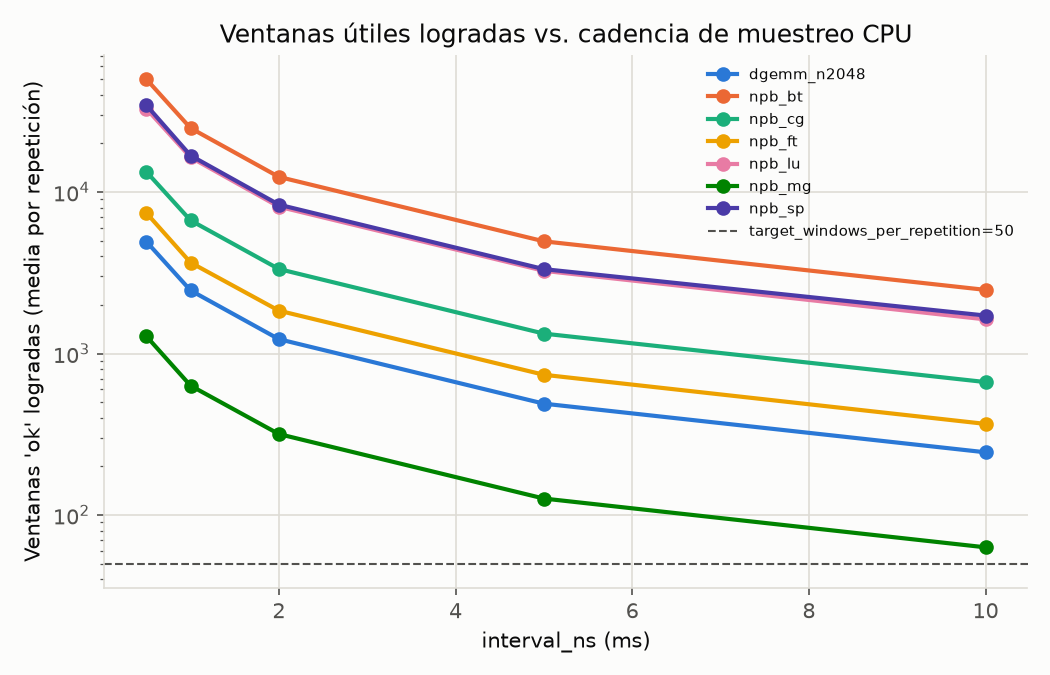
\includegraphics[width=0.85\textwidth]{../plots/interval_ns/windows_ok_vs_interval.png}
\caption{Ventanas \texttt{ok} logradas (media de 3 repeticiones) en función
de la cadencia de muestreo, para los 7 kernels de dataset CPU.}
\label{fig:interval-windows}
\end{figure}

\subsection{Fidelidad del muestreo: el argumento central para 1\,ms}

La Figura~\ref{fig:interval-fidelity} contiene el hallazgo central de este
barrido, pero el promedio simple que la resume oculta una distribución muy
asimétrica -- necesaria de reportar completa para no sobreestimar la
fuerza del argumento. La Tabla~\ref{tab:interval-cv-dist} da la media, la
mediana y el máximo del CV\% del intervalo real (\texttt{sampling\_interval\_cv\_pct}),
sobre las 21 corridas por cadencia (7 kernels $\times$ 3 repeticiones).

\begin{table}[H]
\centering
\caption{Distribución del CV\% del intervalo de muestreo real, por cadencia nominal (21 corridas c/u).}
\label{tab:interval-cv-dist}
\small
\begin{tabular}{@{}lrrr@{}}
\toprule
\textbf{Cadencia} & \textbf{Media} & \textbf{Mediana} & \textbf{Máximo} \\
\midrule
0{,}5\,ms & 1{,}025\,\% & 0{,}154\,\% & 8{,}448\,\% \\
1\,ms     & 0{,}231\,\% & 0{,}098\,\% & 0{,}882\,\% \\
2\,ms     & 0{,}165\,\% & 0{,}155\,\% & 0{,}209\,\% \\
5\,ms     & 0{,}061\,\% & 0{,}055\,\% & 0{,}105\,\% \\
10\,ms    & 0{,}040\,\% & 0{,}038\,\% & 0{,}070\,\% \\
\bottomrule
\end{tabular}
\end{table}

\begin{figure}[H]
\centering
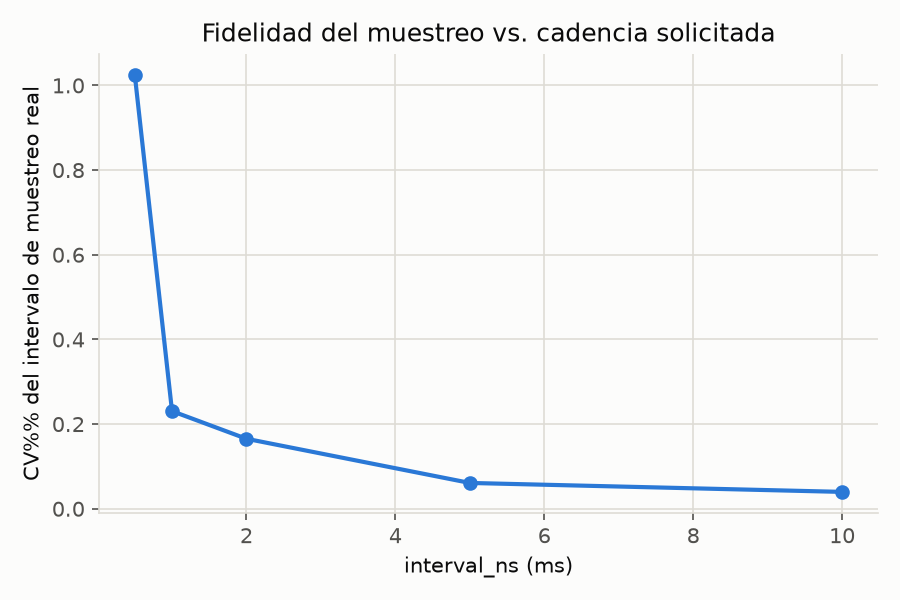
\includegraphics[width=0.75\textwidth]{../plots/interval_ns/sampling_cv_vs_interval.png}
\caption{Fidelidad del muestreo (CV\% del intervalo real vs. el solicitado)
en función de la cadencia. El salto entre 0{,}5\,ms y 1\,ms es la evidencia
central de este barrido.}
\label{fig:interval-fidelity}
\end{figure}

El salto de "más de cuatro veces" en la \textbf{media} (0{,}231\,\%
$\to$ 1{,}025\,\%) está dominado por unas pocas corridas atípicas a
0{,}5\,ms, no por un desplazamiento general de toda la distribución: la
\textbf{mediana} apenas cambia (0{,}098\,\% a 1\,ms vs.\ 0{,}154\,\% a
0{,}5\,ms). Lo que sí cambia de forma clara e inequívoca es el
\textbf{máximo}: 0{,}882\,\% a 1\,ms frente a 8{,}448\,\% a 0{,}5\,ms, casi
diez veces mayor. La lectura correcta no es "la cadencia de 0{,}5\,ms es
en promedio mucho peor", sino que \textbf{0{,}5\,ms es sustancialmente más
vulnerable a eventos ocasionales de interferencia del planificador del
sistema operativo} -- un riesgo de cola, no un sesgo sistemático de toda la
muestra.

Como verificación adicional no reportada en la versión anterior de este
análisis, se recalculó el IPC medio por kernel en cada cadencia respecto a
su propio valor a 1\,ms: la desviación relativa máxima observada, sobre
los 6 kernels CPU con IPC calculable, es de 1{,}93\,\% (\texttt{npb\_sp} a
10\,ms) -- el IPC medido es estable dentro de $\pm$ 2\,\% en todo el rango
0{,}5--10\,ms para todos los kernels probados, así que la cadencia elegida
dentro de ese rango no sesga esta métrica de forma detectable.

\textbf{Conclusión (reformulada)}: 1\,ms es, empíricamente, el primer
punto de la curva en el que el \emph{riesgo de cola} de jitter severo cae
de forma abrupta y donde el IPC medido ya es estable. Es correcto decir
que 1\,ms es un \textbf{valor razonable y conservador, verificado en esta
plataforma}: reduce sustancialmente el riesgo de jitter severo frente a
0{,}5\,ms sin necesitar las ventanas adicionales que 0{,}5\,ms sí ofrece
(aproximadamente el doble, $\sim$20628 vs.\ $\sim$10229 ventanas
\texttt{ok} en promedio sobre los 7 kernels -- corregido respecto a un
valor casi 30 veces menor reportado por un error de conteo en una versión
anterior de este análisis -- una ventaja real, no inexistente, pero
innecesaria frente al objetivo de 50). No es correcto decir que el barrido demuestra que 1\,ms es
"el punto correcto" en un sentido absoluto: no se midió aquí la sobrecarga
propia del instrumento de medición en función de la cadencia, ni la
capacidad de preservar transiciones de carga de duración corta (ambas
quedan como extensiones concretas, no genéricas, de este barrido).
